\documentclass[12pt,a4paper]{article}
\usepackage{times}
\usepackage{durhampaper}
\usepackage{harvard}
\usepackage{graphicx}

\citationmode{abbr}
\bibliographystyle{agsm}

\title{User Interaction Discovery in Virtual Environments}
\student{L.A. Sutton}
\supervisor{W. Li}
\degree{BSc Natural Science}

\date{}

\begin{document}

\maketitle

\begin{abstract}

{\bf Context/Background}
Virtual environments have become a particularly relevant area of computer science in recent years with the rise of social networks such as Facebook, online games, for example World of Warcraft and online means of social interaction, like email. All of these together have enabled many different modes of interactions between users in complex ways which it is important to be able to discover and visualise.

{\bf Aims}
The aim of the project is firstly to produce an effective way of modelling and visualising these interactions, then to use this model and visualisation to discover clustering of these interactions, and the evolution of the model over time with a view to applying the data to draw real-world conclusions.

{\bf Method}
Available literature will be studied in order to see what what current research has been done on data presentation, particularly of networks and also what models are available for the evolution of networks like the ones I will be looking at over time. I will then write an application that implements these as well as allowing me to experiment with alternative visualisations

{\bf Proposed Solution}
A system for visualising multiple modes of interaction will be implemented in Python and a an underlying model will be developed based on available literature. The system will then be developed so that it can identify clustering within the network according to their interaction before giving a quantification of this clustering that can be seen changing over time.

\end{abstract}

\begin{keywords}
user interaction; virtual environment
\end{keywords}

\section{Introduction}

\subsection{Project Description and Purpose}
In this project I have taken virtual environments to mean any environment in which users will interact in a virtual network. This broad definition will include everything from online games in which users interact in a three dimensional virtual world and can interact with each other in multiple complex ways to emails within an organisation which may simply include information being disseminated from a central source.

This wide variety of environments provide many different ways in which users can interact which I have called modes. These modes can then be categorised, for example, if they represent a single or an ongoing interaction, or depending on whether the interaction is one to one, many to one or many to many.

I can then use properties of my visualisation such as the colour or size of nodes in a graph or their distance or by introducing some graphic link between them to visualise these different modes.

\subsection{Project Deliverables}
Firstly, my project will deliver a system that is able to visualise the interactions between users in real time. It will contain visualisations that distinguish between different modes of interaction, with configuration that allows the user to change which modes of interaction are represented. The system will also be able to model a time evolution caused by the interactions between the users. It will then also be possible to visualise this time evolution as well as quantify this evolution in useful metrics. Finally the system will allow visualisation of clustering of the user according to the interactions that they make, and will allow visualisation of the changes in clustering over time that result from the evolution of the system.

\subsection{Current Work}

\subsubsection{Social Network Visualisation}
%There has already been much work carried out on the visualisation of the relationships and interaction within virtual networks. Previously, low level visualisation tools have been developed specifically for the purpose of visualisation of data within a network \cite{heer2005prefuse}. These have been designed so that they have the flexibility to accommodate a range of presentation techniques. The these tools have been use to build fully functional tools designed to be used by users with little technical experience. For example an application has been made that visualizes data from the 'Friendster' social network and allows this data to be viewed in different ways to facilitate discovery of previously unknown information\cite{heer2005vizster}. They allow the user to modify the layout themselves by simply intuitive controls and use colour and position to make the visualisation more clear. There have also been tools developed that, as well as visualising the data provide tools for detailed statistical analysis providing numerical data on graph clustering and community identification\cite{borgatti2002ucinet}. However, these tools have focused on the analysis and visualisation of snapshots of data remaining static, rather than data sets that evolve over time.
Network visualisation is already a science with a long history, especially since being able to use computers to position and draw the output. There are currently low-level tools that exist with the intention that they have the necessary flexibility to accommodate a wide variety of visualisation styles and techniques \cite{heer2005prefuse}. As well as this, there are tools that exist to provide numerical analysis \cite{borgatti2002ucinet}. However, these tools have focused on the analysis and visualisation of snapshots of data remaining static, rather than data sets that evolve over time. These have also previously been used to build ways of visualising social network data from Friendster \cite{heer2005vizster} in order to facilitate discovery of more information than would be apparent from other ways of looking the data, as I hope to.

\subsubsection{Information Presentation}
There is also a wide variety of information on the presentation of data on computer screens. One particularly popular model can be summed up as 'Overview, Zoom, Filter' \cite{shneiderman1996eyes}. In this it is suggested that the initial view of the data should be a movable field of view with emphasis on allowing the user to gain an 'overview' of relevant data and identify areas which will be of interest. Specific areas of interest can then be zoomed in on preserving the context of the overall picture before extra information of areas of interest can be viewed possibly by clicking on them. This paper also talks about things such as the importance of smooth display updates and responsiveness to user input. This is built upon by the ideas of making information more clear by distorting the 'presentation space' \cite{carpendale2001framework}. This is the method used in Vizster and can be seen in common usage in many different data visualisation applications. It imagines that the virtual space in which the data is presented is a real material that can be stretched and viewed through a movable lens as necessary to make the relevant areas of the information more clear. These ideas area also expanded on further to see what kinds of lenses are suitable for which purposes, and suggests a mathematical framework for implementing such a lens \cite{leung1994review}. Contained in all of these articles on visualisation are also many suggestions for evaluation of data presentation on computers for example by the ability to maintain context between switching between the three areas on the 'Overview, Zoom, Filter' model and the responsiveness to user input that is possible.

\subsubsection{Graph Drawing}
There is also previous literature on the drawing of graphs in aesthetically pleasing ways. Almost all current research makes use of a force directed spring layout. In this algorithm, each node is modelled is repelling each other node and the edges between them are modelled as springs\cite{fruchterman1991graph}. Included in these papers are suggestions for the strength of the attractive and repulsive forces different distances and the size of graph that this can be expected to create. However, this algorithm doesn't scale well with rapidly increasing numbers of vertices. It has been pointed out that with a large number of nodes, calculating the layout in this way is very expensive in terms of computing power. However, with the correct optimisations it is possible to reduce the complexity to $o(nlog(n))$ \cite{barnes1986hierarchical}.

\subsubsection{Modelling Social Networks}
The ability to produce networks of relations and interactions from many different data sources is also explored in a variety of different papers. For example, networks of social interaction have been produced from a history of email correspondence within an organisation \cite{fisher2004social}. Here other relevant ideas are explored such as the privacy implications of collecting data on a large scale and the ability to reconstruct the whole graph from only partial data. The same has also been achieved using the transcript of an internet relay chat \cite{mutton2004inferring} again struggling with the problem of reconstructing a complete graph from partial data. It is then further shown that the same method including the temporal decay of relationships can be applied to other sources of relationship information involving over time such as the plays of William Shakespeare.

\subsubsection{Categorisation of Interactions}
Previous reserach has also explored categorisation of interactions by their characteristics. This has mainly in the past been applied to social iterations writing 3D virtual environments in which people interact as virtual avatars, referred to as Networked-Virtual Environments. One particular application of this is games \cite{manninen2000interaction}. Here we can see that there is more than one way of categorising interactions, one way being based on their purpose. These papers also show how it is possible for many different modes of interaction to happen symeltaniously. It is possible to use communicative action theory to categorise interactions by their purpose, this is extended in other papers by comparing interactions in a selection of game environments \cite{becker2002social}. Extending this to other environments such as the social network, other papers show how much of the interaction that goes on writhing a virtual environment is hidden from the user. We can see just how much data website such as Facebook collect about us including in our making interactions which we wouldn't normally consider meaningful \cite{schneier2010taxonomy}

\subsubsection{Evolution of social networks}
Ideas of the behaviour of users in social networks have been the subject of many different papers. This includes homophily \cite{adamic2003social} which is the idea that people on social networks tend to associate with people who are similar to themselves in terms of age, political views etc. Work has also been completed on the behaviours of users within a social network and the ways in which interactions can spread behaviour across networks of people represented as graphs. It has been suggested that this can be explained using a virus like model \cite{centola2010spread} in which users pass between susceptible, infected and recovered states, analogous to a computer-virus or a real virus.

\subsubsection{Detection of clustering}
Detecting features of social networks that are not immediately apparent is also extremely important. We can see that algorithms have been developed that aim to detect communities, related to clustered sections of graph representations of these networks \cite{newman2004fast}. These algorithms can be applied to real world networks with a good degree of success reported in identifying the same communities that the users themselves identify with.

\section{Design}

\subsection{Functional Requirements}

\begin{table}[htb]
\centering
\caption{Functional Requirements}
\vspace*{6pt}
\label{tab:requirements}
\begin{tabular}{c p{11cm}}\hline\hline
Requirement Number & Description \\ \hline
1 & Implement a basic system for modelling simple user interactions in a virtual environment \\
2 & Implement a visual output for this model \\
3 & Expand the implementation to cover multiple modes of interaction \\
4 & Implement an evolution of the model over time with the ability to quantify the evolution \\
5 & Implement a grouping/clustering of users in the virtual environment based on their interactions \\
6 & Implement visualisation of the clustering of users \\
7 & Implement  a way of outputting data that can be shown to have real-world applications
\end{tabular}
\end{table}

\subsubsection{Requirement 1}
The system should be able to model basic user interactions for example writing on walls of a social network. It should do this by forming a graph in which the users are represented by nodes and the relationships between them by edges. Interactions will then take place between nodes connected by edges which are then remembered by each node.

\subsubsection{Requirement 2}
The system will provide a visual output that represents the interactions, users and relationships from the model in requirement 1. This will be done by drawing a graph with the users represented by nodes and the relationships between them by edges with different features of each being represented by the properties of these. For example, relationship strength could be shown by edge length or age by node colour.
\begin{figure}[htb]
\begin{center}
\caption{An example visualisation}
\label{fig:visualexample}
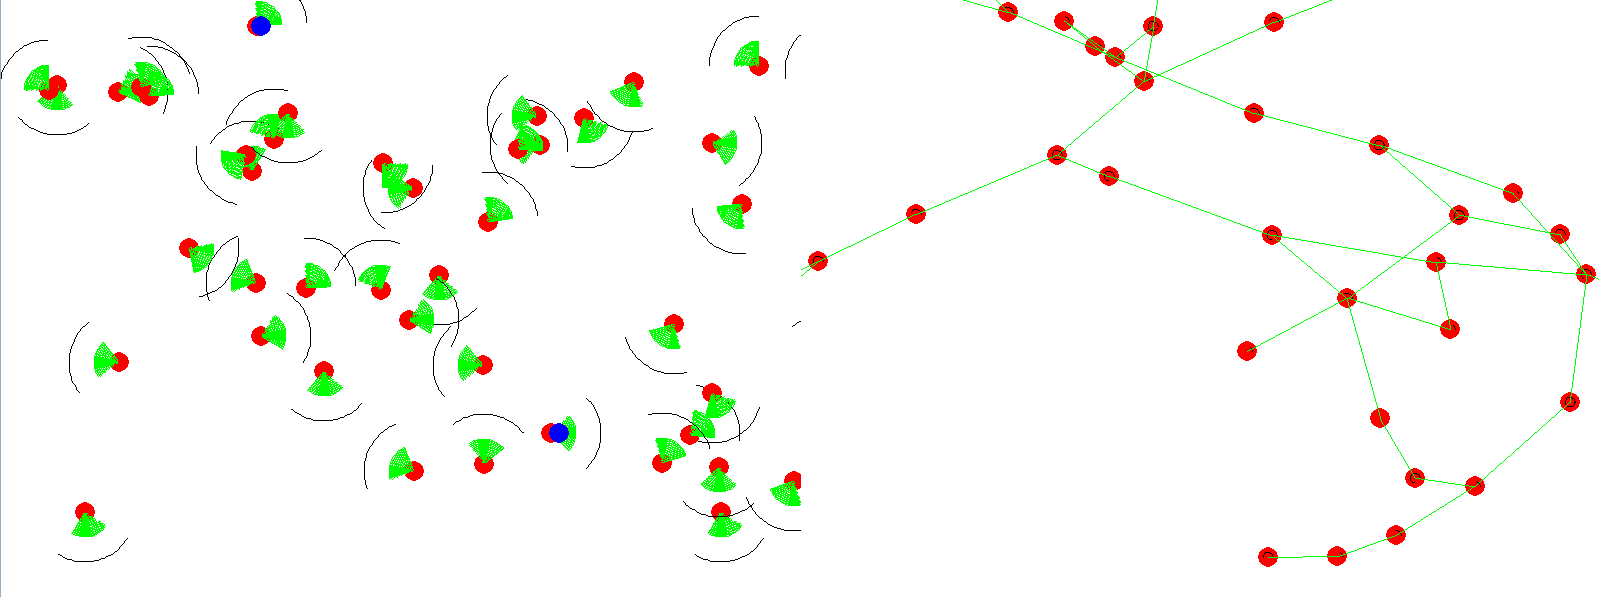
\includegraphics[width=6in]{screen}
\end{center}
\end{figure}

An example of visualisation from a mock-up can be seen Figure \ref{fig:visualexample}. This also includes on the left a view of users within a three dimensional environment that might be implemented in requirement 3.

\subsubsection{Requirement 3}
\begin{figure}[htb]
\begin{center}
\caption{Interaction Types}
\label{fig:types}
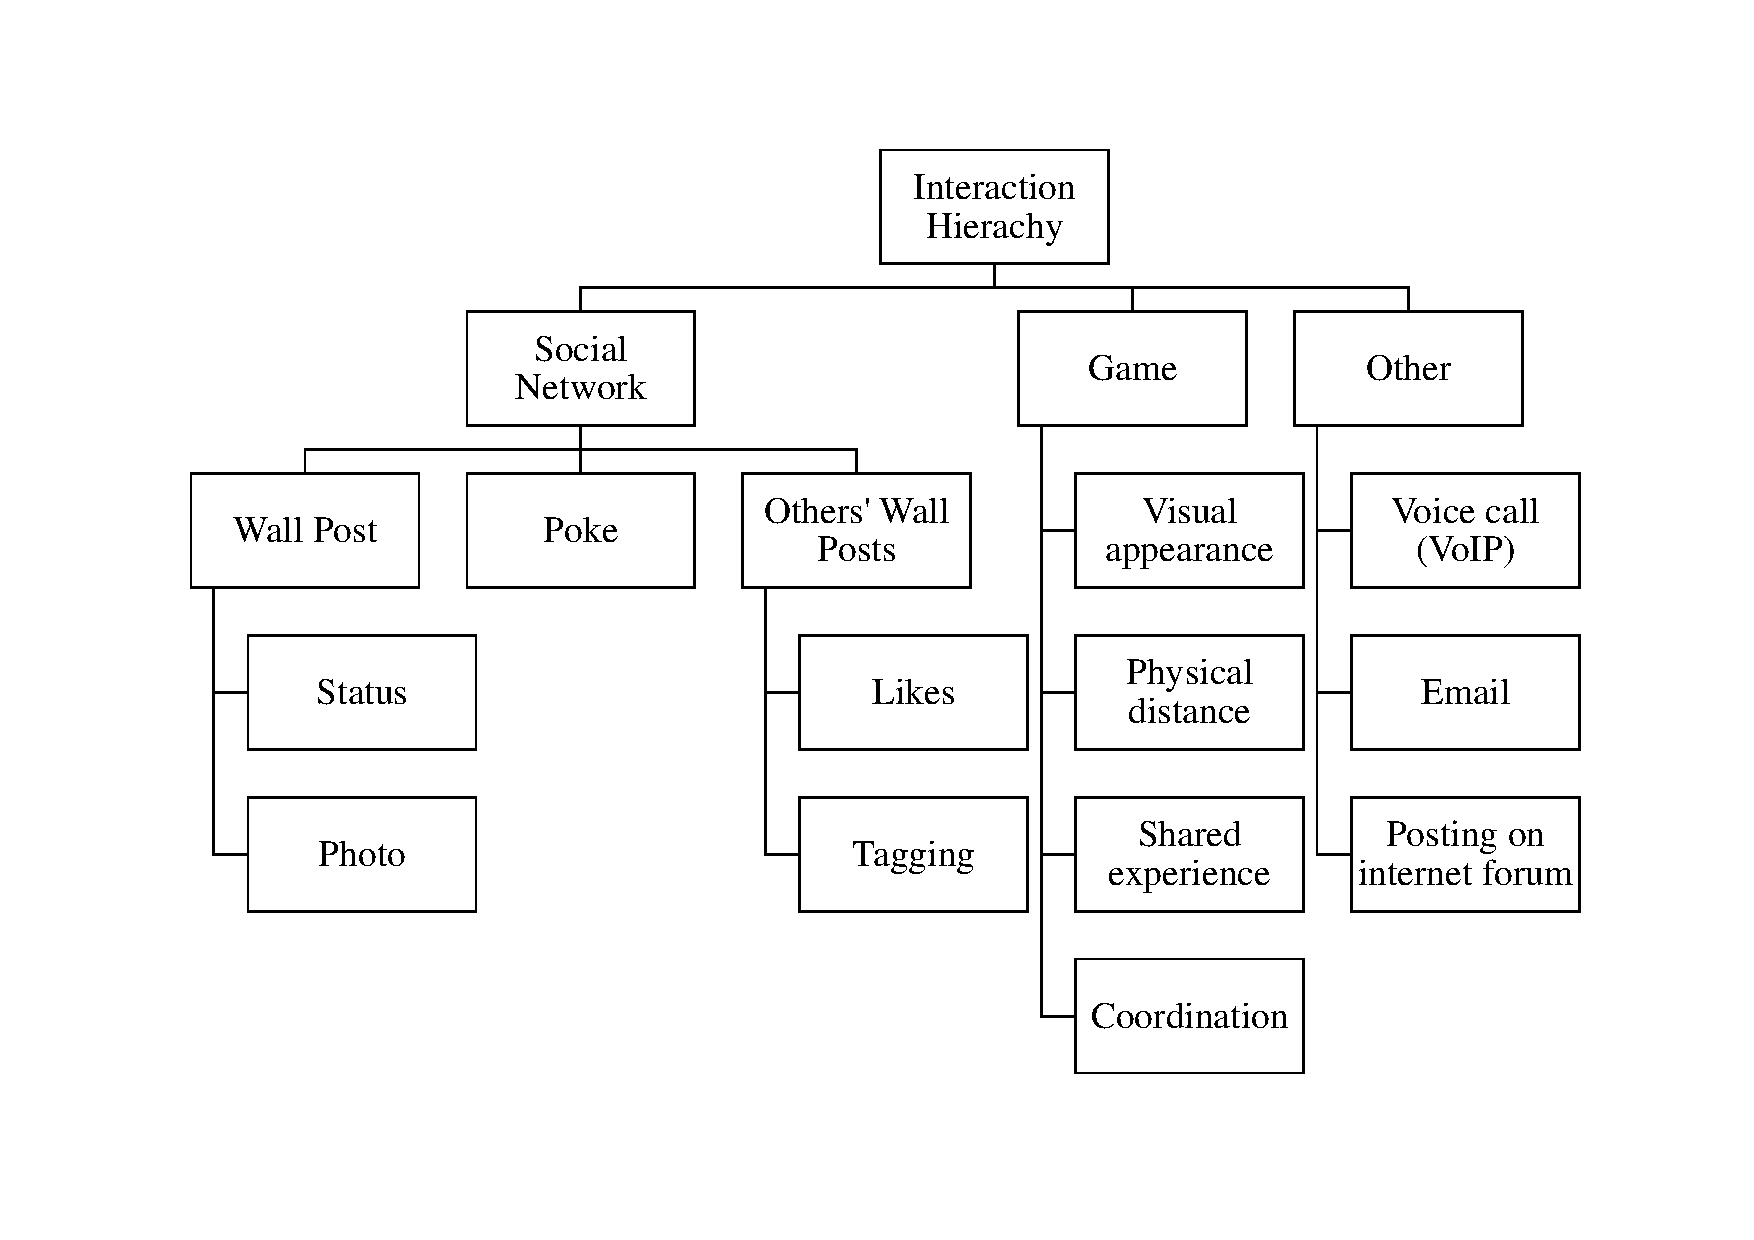
\includegraphics[width=6in]{InteractionTypes}
\end{center}\end{figure}

\begin{figure}[htb]
\begin{center}
\caption{Interaction Modes}
\label{fig:modes}
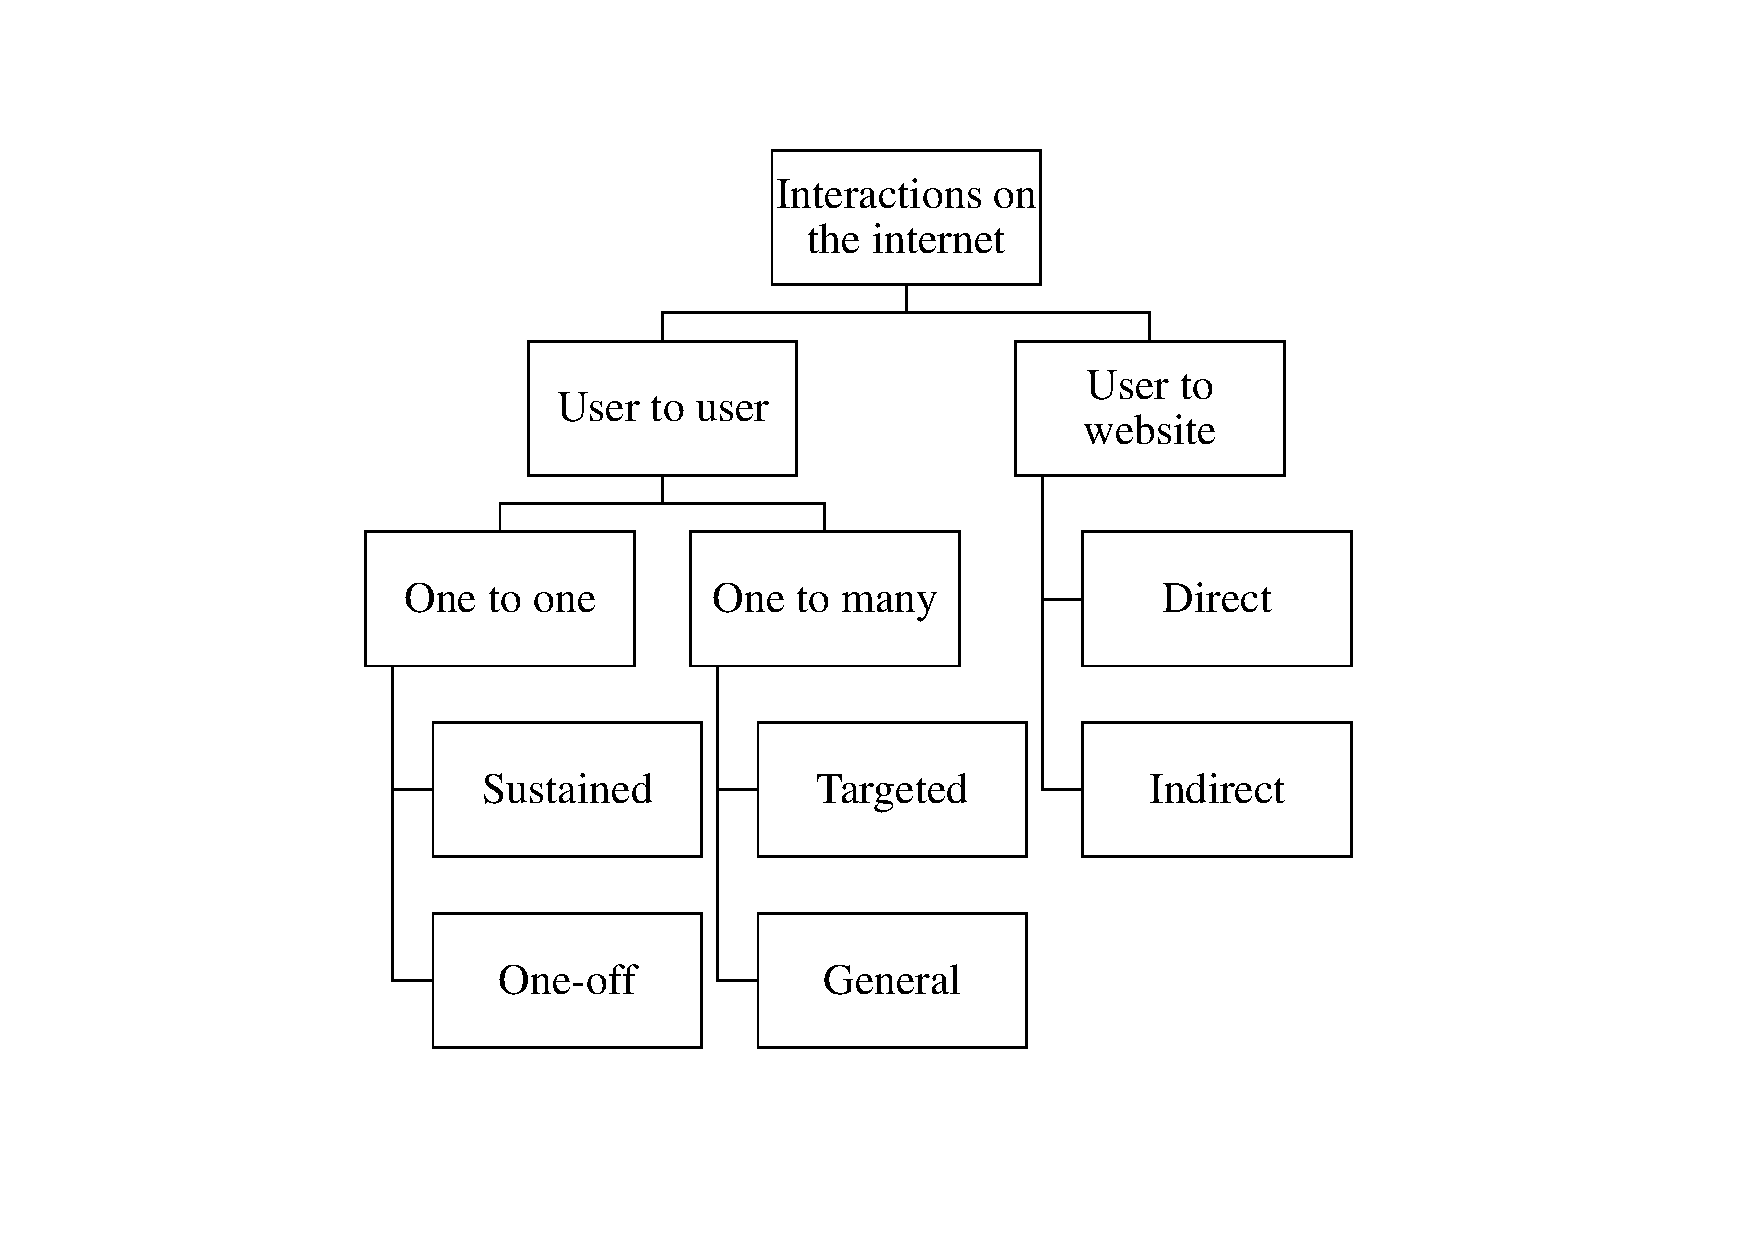
\includegraphics[width=6in]{CategorisationsInteractions}
\end{center}
\end{figure}

When considering multiple modes of interaction I found that there was little current literature linking interaction modes with categorisations. This lead me to then design two hierarchies. The first in order to categorise what different interactions were possible within the virtual environments I was considering, the second to categorise them in terms of how they could be represented.

Initially I produced Figure \ref{fig:types} in order to categorise the types of interactions that were possible. These came largely from personal experience and I produced this in order to help me consider what categories of interactions it would be necessary to visualise.

This lead me to Figure \ref{fig:modes}, which are the modes of interaction that I will be visualising. The model will then be expanded to cover as many of these as possible, allowing experimentation both with how these might affect the evolution of the model over time.

\subsubsection{Requirement 4}
The model will evolve in three ways, firstly the people will move around in their 3D environment. They have random motion around the environment and aren't allowed to move out of its bounds.

The second way that the model will evolve is in the change in relationship strength between the pairs of people. This will be affected by the interactions between the users of the relationships being affected and will also be affected by time as people who don't interact lose relationship strength.

\subsubsection{Requirement 5}
The model will be designed in such a way that the interactions over time will cause relationships between the users to change. This will in turn mean that the users cluster themselves according to their interactions and their starting states.

\subsubsection{Requirement 6}
The system will enable a visualisation of the clustering of users and the way that this clustering changes over time. This should be able to be configured by the user to allow clustering according to different metrics. This visualisation should also allow the user to see how clustering has changed over time as the model evolves.

\subsubsection{Requirement 7}
The system should output quantitative data about the clustering and evolution of the model over time which can be given real-world applications. Algorithms must be found which can represent the system at different times.

\subsection{Architecture}

\begin{figure}[htb]
\begin{center}
\caption{Class Diagram}
\label{fig:class}
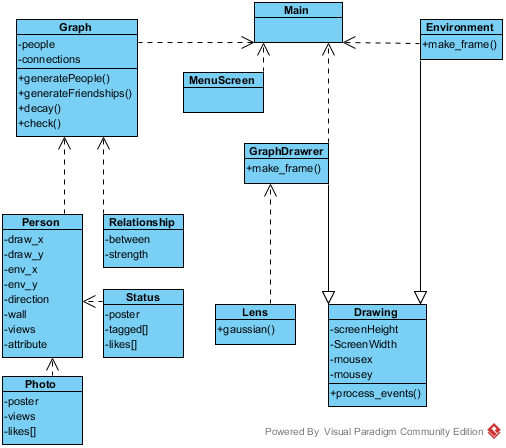
\includegraphics[width=6in]{Classpng}
\end{center}
\end{figure}

\subsubsection{Main}
The MainController class is the one that coordinates the setup and initialisation of the program along with choosing what interactions will be represented. This also coordinates the synchronisation of frames between the two Drawing objects in order to draw them together.

\subsubsection{MenuScreen}
The MenuScreen allows the user to configure the visual output in different ways. For example, they can change the colour or map different aspects of the model or affect which aspects of the user or relationship between users is represented by which aspect of the visual output. For example the size of a node could represent a user's age, or the number of posts on their wall. The menu is implemented using the Tkinter toolkit for python which is a common and popular way of adding forms to python applications. The MenuScreen passes the selected options back to Main which then creates the visual output with the selected options.

\subsubsection{Graph}
The Graph object contains a list of Person objects (people) and a list of Relationship objects (connections). This stores all of the people that are being considered in the virtual environment and the relationships between them. This object also handles the initial generation of people through the generatePeople() method which randomly generates a predetermined number of people with random attributes. the generateFriendships() method the determines a predetermined number of relationship objects between the people with random strength.

The decay method if called will iterate through the relationships and modify them all by a set amount. This is called in order to simulate the decay of relationships over time between pairs of people who do not interact. The check() method will again iterate through all relationships and check that they are all legal. That two relationships haven't been created between the same pair, it will also remove relationships once they fall below a certain level.

\subsubsection{Person}
A Person class represents a person in the virtual environment and forms part of the graph. The person object contains all the attributes of the person including the draw\_x and draw\_y fields which represent the point at which this person is being represented in the graph view and the env\_x and env\_y fields at which this person currently is in the 3 dimensional environment. The direction field then applies to the direction in which this person is looking in the 3D environment.

For the social side of the virtual environment, the person object includes a wall, which functions in the same way as a wall in Facebook with the photos and statuses being modelled on the wall. Finally for the social network each person has a field which I have called views. This represents the persons social or political views that other people might agree/disagree with and are represented in social network statuses

\subsubsection{Relationship}
A Relationship object represents the relationship between two Person objects. The between field contains a tuple representing the people the Relatinonship is between and the strength field indicates the strength of the feeling between the two people

\subsubsection{Status}
A status is simply an object that can be posted on a wall. It contains as the poster field a reference to the Person object who posted it on the wall. The views field 
represents the views of the poster which the person who looks at it might either agree or disagree with and finally the likes[] field contains references to the Person objects who have interacted with the status by liking it.

\subsubsection{Photo}
Similar to a status the Photo object again represents something posted on a wall. The only difference this time is that it contains in its tagged[] field a list of the people who are tagged in the photo, changing their relationship with the tagger, the poster and the person on who's wall the photo was posted.

\subsubsection{Drawing}
The drawing object contains the methods and fields that are common between the two types of drawing in the representation. The constructor fills the screenHeight and screenWidth fields and then every time a drawing calls the process\_events() method the object checks if it should close the window and exit of if a key has been pressed changing the representation of and then updates the mousex and mousey fields with the current mouse position

\subsubsection{GraphDrawerer}
This inherits from the Drawing object and draws a graph of nodes and edges representing all of the people currently being considered int he virtual environment and the relationships between them. It constructs the layout of this graph by means of a force directed drawing algorithm to place the nodes in the clearest possibly arrangement in a reasonable amount of time. It does this by assuming that there is an attractive force of $x^2/k$ along each of the edges where $x$ is the distance and $k$ is a constant and a repulsive force of $k^2/x$ between each of the pairs of nodes. Several iterations of this are taken as each node is moved by the resultant 'force' on it, changing position less each time until a local minimum has been reached. The make\_frame() function then produces the next frame of the visualisation that can be rendered with others.

\subsubsection{Lens}
The lens object contains one method associated with the drawing of the graph as distorted by an imaginary lens. It calculates the result of a gaussian function based on the distance between two poiwnts. The function used is
\begin{equation}
f(x)=(1/(\sigma\sqrt(2*\pi))(-(x-b)^2/(2c^2)).
\end{equation}
This can then be used to separate points for closer inspection.

\subsubsection{Environment}
This class is responsible for drawing a representation of the characters in the 3D environment. it takes the env\_x and env\_y fields from the Person class and uses this and the direction to draw the people at these points. Calling the make\_frame() then produces the next frame of the visualisation to be rendered alongside another.

\subsection{Tools Used}
This project was built using Python 3.4. I chose to use python because it was a language with which I was already familiar and I felt that it would enable to me to quickly develop the necessary model and visualisation. I also believed that the speed of languages such as Java was unnecessary as I planned to produce only two dimensional graphics as output and there was no major computation required for the evolution of the model. The development in python was conducted using the PyCharm IDE which again I was already familiar with and was sell suited to my project.

The graphical output was produced using the PyGame. This was used because it would be easier to use than OpenGL to quickly experiment with different graphical outputs and because it makes used of optimised C code this means that the speed of the graphical output shouldn't slow down any of the computation relating to the model.

Finally I also made use of Numpy. This was used for easier handling of arrays, particularly when calculating positions for layouts of nodes within the graphical output.

\section{Evaluation}
The system will be evaluated in two ways, first against the requirements that I have listed here and second it will be compared to systems that already exist in order to see if it can offer any benefits over those systems or falls short of them.

First I will evaluate the finished system according to each of the functional requirements I have listed here individually. I will compare my final application to the requirement listed and check to make sure that all of the criteria have been met or whether it has been necessary to compromise and I have failed to meet the requirements. This will also allow me to see how well my I formed my requirements initially, and evaluate how my plan changed over time.

Secondly, I will spend time comparing my system to other systems that are already available. There are many of these that apply specifically to social networks such as Vizster as I have previously mentioned but there are many other tools available for free online which offer visualisation of social network graph data. I will take a selection of these tools and, compared to my own application, see how well they fulfil the aims of my project. This will allow me to determine where my application could have been improved in order to better meet its aims and also compare it to alternative approaches where these are taken.

\section{References}

\bibliography{projectpaper}


\end{document}
